\begin{figure}[t]
\uwsinglespace
\begin{center}
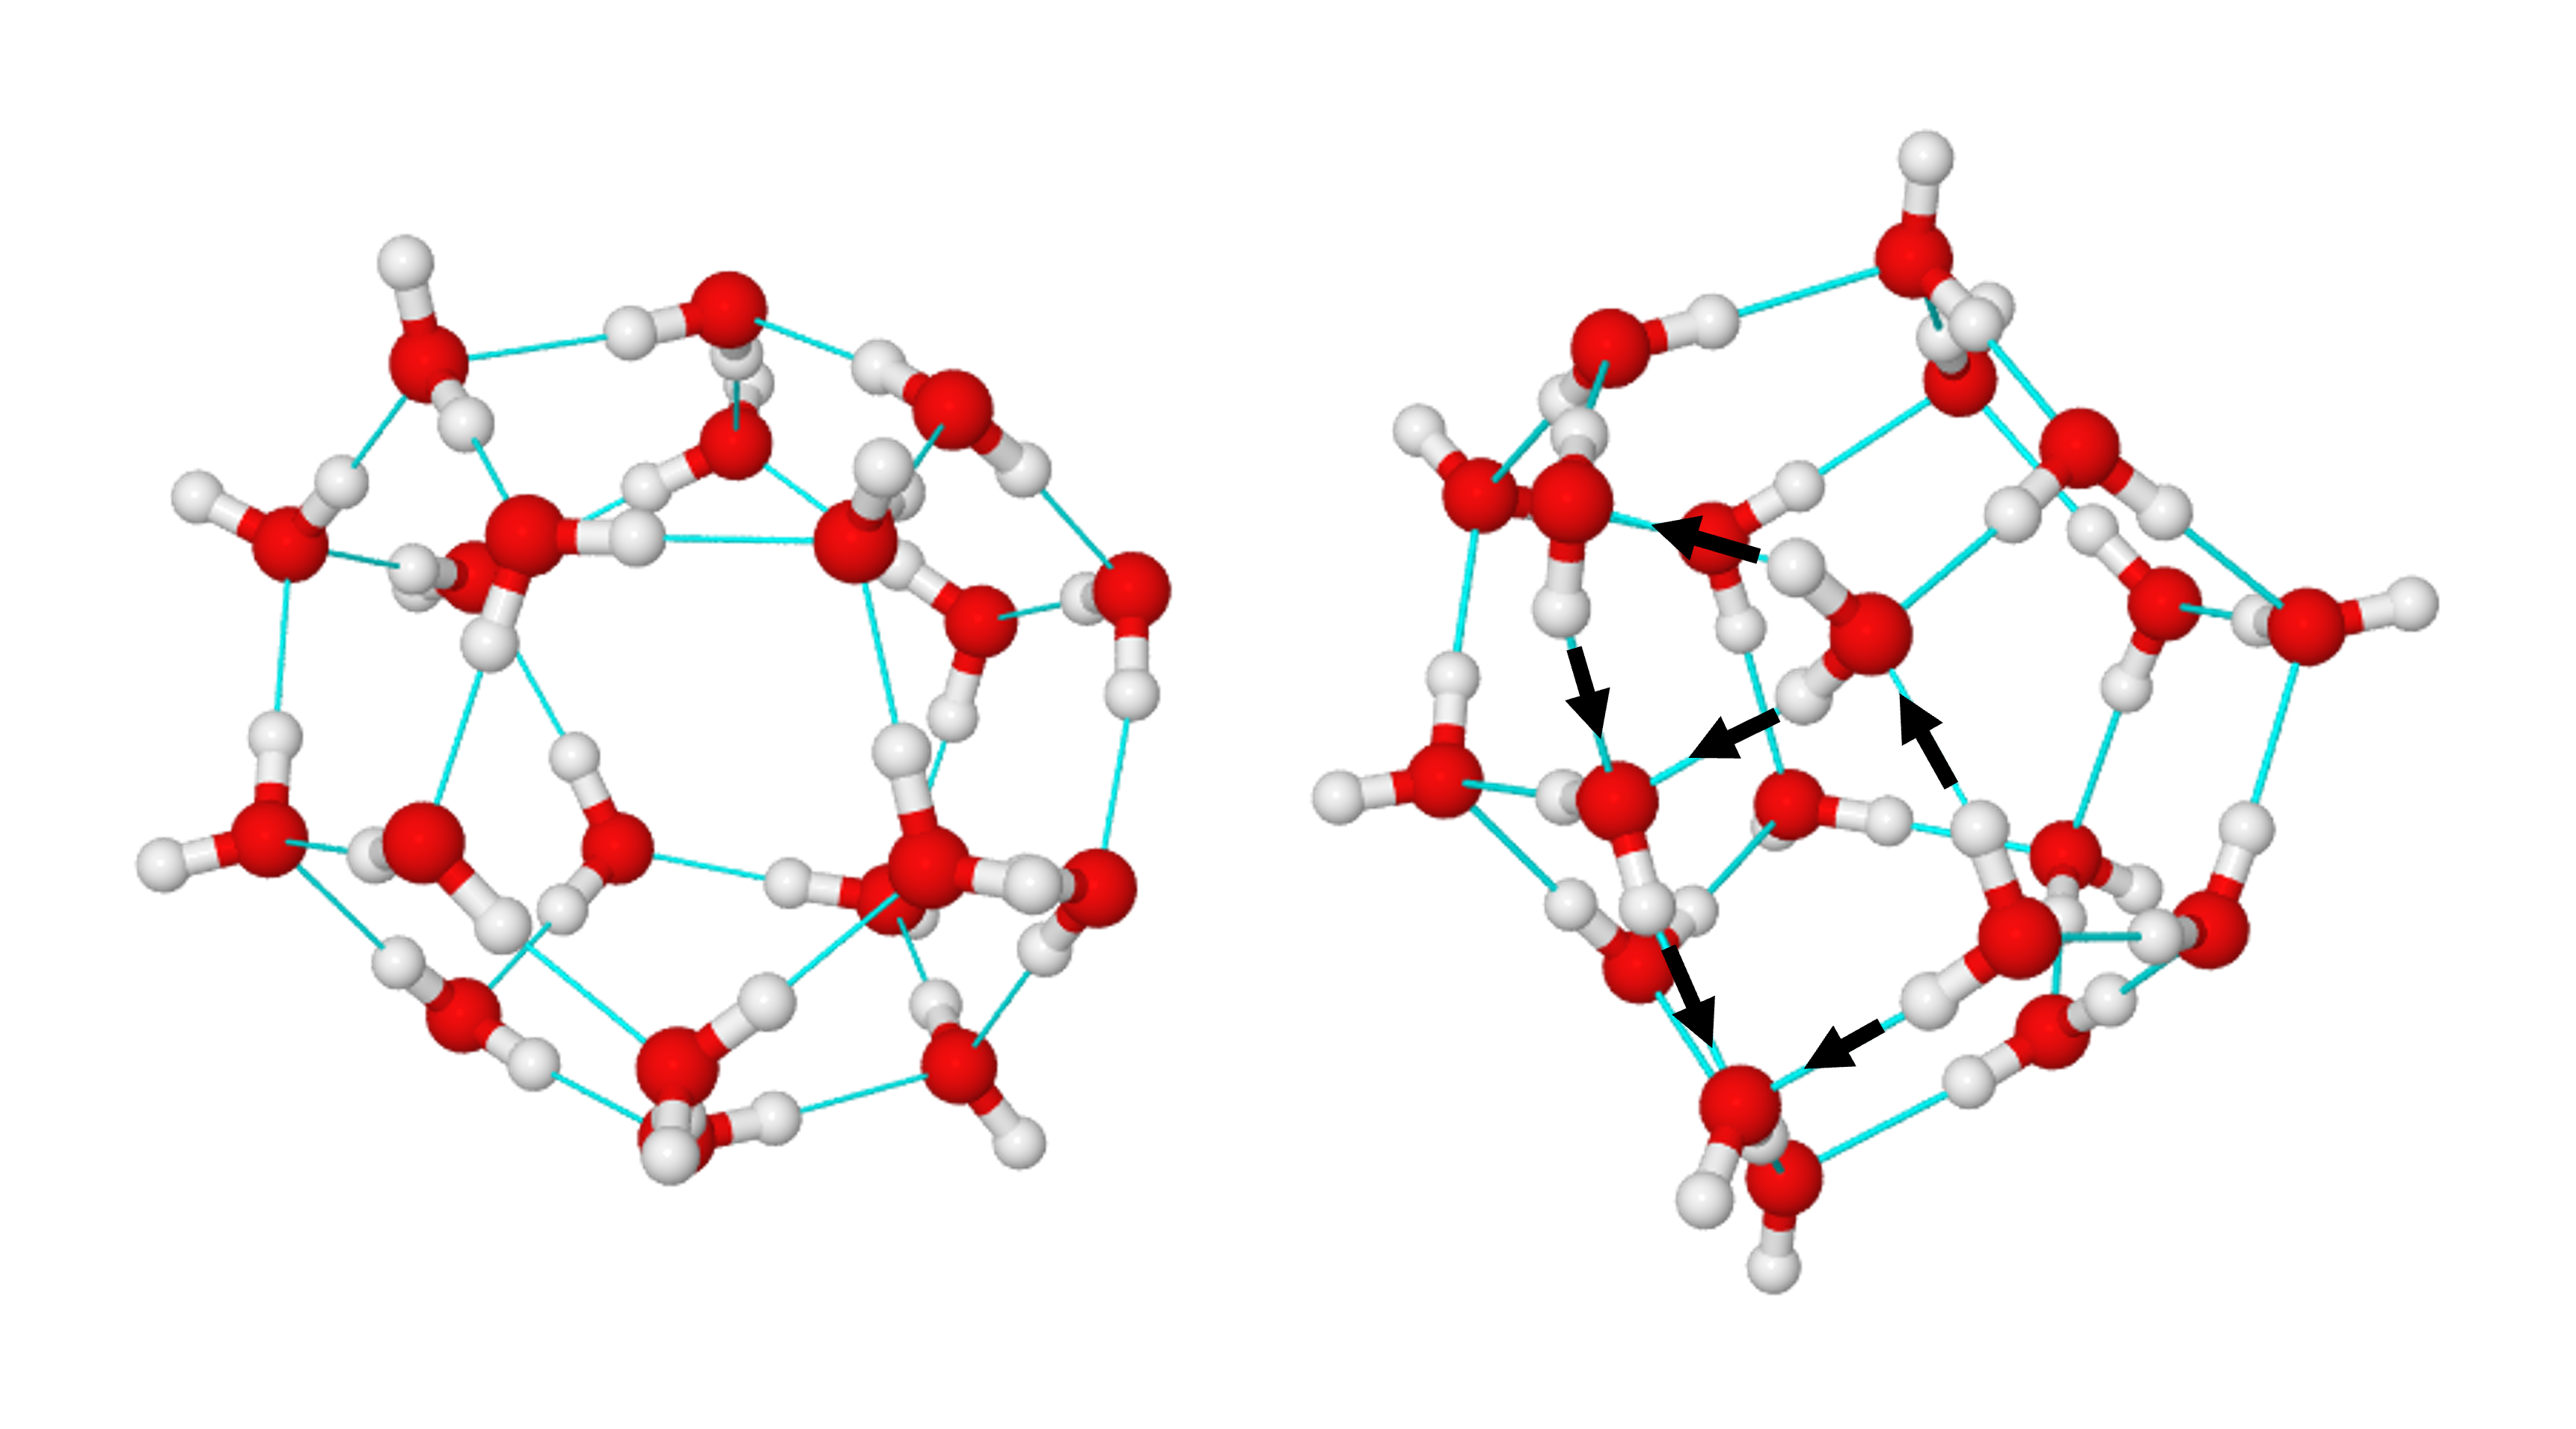
\includegraphics[width=\textwidth]{Figures/Chapter_6/clathrate_distortion_comparison.png}
\end{center}
\begin{spacing}{1.0}
\caption[Examples of a stable \ce{(H2O)_{20}} clathrate cage (left) and one of the most common defects, which occurs when a candidate clathrate structure collapses to a different hydrogen bonding arrangement. The arrows show that a free OH bridges one of the 5-membered rings in \ce{(H2O)_{20}}, resulting in fused 3- and 4-membered rings.]{Examples of a stable \ce{(H2O)_{20}} clathrate cage (left) and one of the most common defects, which occurs when a candidate clathrate structure collapses to a different hydrogen bonding arrangement. The arrows show that a free OH bridges one of the 5-membered rings in \ce{(H2O)_{20}}, resulting in fused 3- and 4-membered rings.}\label{fig:MBE_III_F3}
\end{spacing}
\end{figure}